\section{SAW as a method of fluid atomization}
\label{sec:saw_vapour}

Using SAW technology to produce small scale fluid atomization devices is not a recent idea. 
The concept was already demonstrated by \Citeauthor{kurosawaSurfaceAcousticWave1995}\cite{kurosawaSurfaceAcousticWave1995} in 1995, but mass produced SAW-based atomizers are still not commercially available, likely due to challenges related to the precision engineering required for mass production.

However, because of the many possible applications of low-power, compact fluid atomizers such as inhalation therapy \cite{qiMiniatureInhalationTherapy2009a}, thin film deposition \cite{murochiDepositionThinFilm2007} or nanoparticle synthesis \cite{alvarezRapidGenerationProtein2008}, there is still a substantial interest in improving the technology and optimizing it for production.

Depending on the boundary conditions various acoustofluidic effects can take place during the interaction between SAW and a fluid \cite{winklerSAWbasedFluidAtomization2015a}.
The geometry of the liquid volume has a large on the physical phenomena at play and may result in different atomization regimes, some of which are not entirely understood yet \cite{collinsAtomizationThinWater2012,huangExperimentalResearchSurface2022}.
Describing these highly complex microfluidic phenomena in their entirety is beyond the scope of this work, which is why the following section will focus on the general principle of fluid atomization without going into detail about the governing equations.

When the SAW hits the liquid surface, it is diffracted into the liquid volume at the \emph{Rayleigh angle} $\theta_\text{R} = \sin^{-1}(c_\text{l}/c_\text{SAW})$, which depends on the speed of sound in the liquid $c_\text{l}$ and the propagation speed of the SAW $c_\text{SAW}$ and is $\sim\SI{22}{\degree}$ for water.
The acoustic radiation \emph{leaked} into the liquid causes a longitudinal pressure wave which leads to a bulk recirculation of the liquid known as \emph{acoustic streaming}.

This phenomenon is useful for a variety of applications, such as the mixing of liquids or the transport of particles in a liquid, but is not primarily responsible for the atomization process.
However it has an important influence on the geometry of the liquid volume, which has a significant impact on the droplet formation, as mentioned earlier.

The main driving force behind the atomization process is the capillary waves that form on the liquid surface.
The vertical surface displacement observed for Rayleigh waves is only around \SI{10}{\nano\meter}, however particles are accelerated at around \SI{e7}{\meter/\second\squared}.
If enough power is used, the capillary waves can be amplified to a point where they overcome the surface tension to break and form droplets.

\begin{figure}[htbp]
    \centering
    \makebox[\textwidth][c]{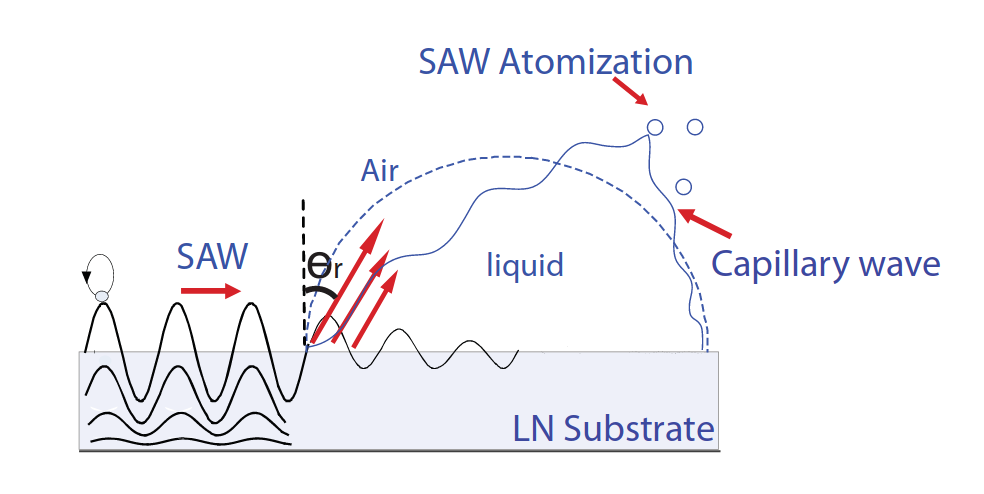
\includegraphics[width=0.7\textwidth]{images/Screenshot-20230211174610-984x494.png}}
    \caption{Schematic depiction of the SAW atomization process. The wave hits the and causes capillary waves on the liquid air interface. \emph{LN} stands for \emph{lithium niobate}, a commonly used piezoelectric material. \cite{aishaqiInvestigationSAWAtomization2009}}
    \label{fig:atomization}
\end{figure}

The exact relationships between the excitation frequency, the capillary wave frequency and the droplet size are not fully understood yet and different models haven been proposed over time.
The main influences in the relationship appear to be the liquid viscosity, the liquid surface tension and the liquid density \cite{aishaqiInvestigationSAWAtomization2009,huangExperimentalResearchSurface2022}.
The latest findings suggest that that the droplet size $D$ is in the same order of magnitude as the wavelength of the capillary waves $\lambda_\text{c}$, which seems to be inversely proportional to the excitation frequency $f$ \cite{collinsAtomizationThinWater2012}.
$$
    D \sim \lambda_\text{c} \sim \frac{1}{f}
$$

Different SAW atomizers differ primarily in how they supply liquid to the atomization area, examples including a \emph{droplet-on-demand} system, where the liquid is supplied by a syringe pump, or a \emph{continuous flow} system, where wetted laboratory paper is placed  on the substrate and the liquid is supplied by a reservoir, with atomization taking place at the meniscus that forms at the edge of the paper \cite{winklerSAWbasedFluidAtomization2015a}.

The method of liquid supply developed at our institute uses a small capillary channel that is mill-cut directly into the substrate, which has direct contact to a liquid reservoir, filling itself using the capillary effect.
This method is very simple and does not require any additional components, which makes it very suitable for mass production.
Ongoing research explores the influence of channel geometry on the atomization process \cite{kapplAkustischInduzierteVernebelung2022}.

